\chapter{ML}

\section{Artificial neuron}

Artificial neurons, also called perceptrons were developed in the late 1950s and early 1960s, firstly introduced by Rosenblatt in his paper \cite{perceptron}. His idea was to develop a model capable of simulating the activities present in the human brain cell, in order to create artificial intelligence. As it turned out, simulating the brain using such a simple model as the perceptron is impossible. However, later research discovered a considerable potential in the field of classification and regression, which lead to design of modern artificial neural networks as we know them today.

Perceptron is a simple probabilistic model, which takes several weighted real inputs and produces one real output.

\vspace{3mm}

\begin{figure}[h]
\raggedright
\begin{subfigure}{.35\textwidth}
  \centering
  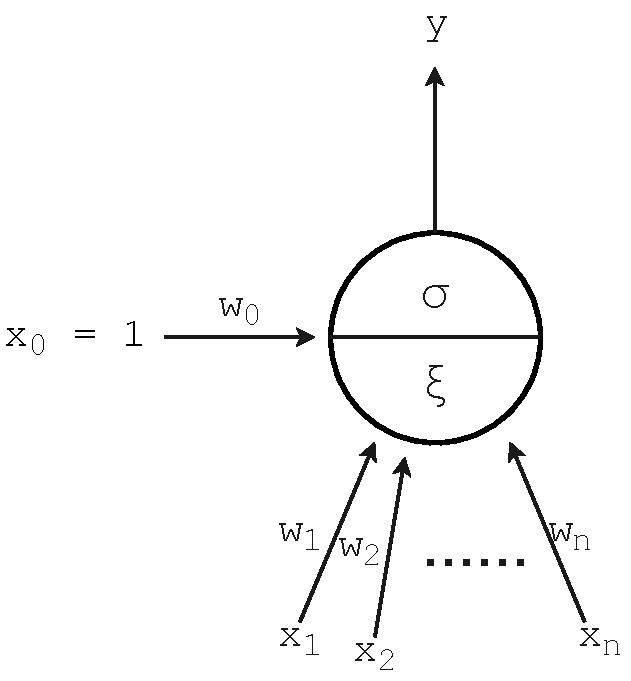
\includegraphics[width=\textwidth]{tex/images/perceptron}
  \caption{Artificial neuron}
\end{subfigure}%
\hfill
\begin{subfigure}{.55\textwidth}
  \centering
  \begin{itemize}

	\item $x_1, \cdots, x_n$ are real \textbf{inputs}
	\item $x_0$ is always equal to 1
	\item $w_0, w_1, \cdots, w_n$ are real \textbf{weights}
	\item $\xi$ is inner \textbf{potential}, \\$\xi = w_0 + \Sigma_{i=1}^n w_i x_i$
	\item $y$ is real \textbf{output} given as \\ $y = \sigma(\xi)$
	\item $\sigma$ is an \textbf{activation function}

	\end{itemize}
\end{subfigure}
\end{figure}

\section{activation}

An activation function $\sigma: \mathbb{R} \rightarrow \mathbb{R}$ is applied to the inner potential $\xi$, and it defines the output value of perceptron. It introduces a powerful tool into machine learning, and that is \textbf{non-linearity}. Without the activation, the potential by itself is a simple polynomial of a degree of one. That would limit the learning ability of the neural network into being a simple regression model. However, using different activation functions, we can adapt the model to more complicated mappings.

\begin{figure}[h]

\centering
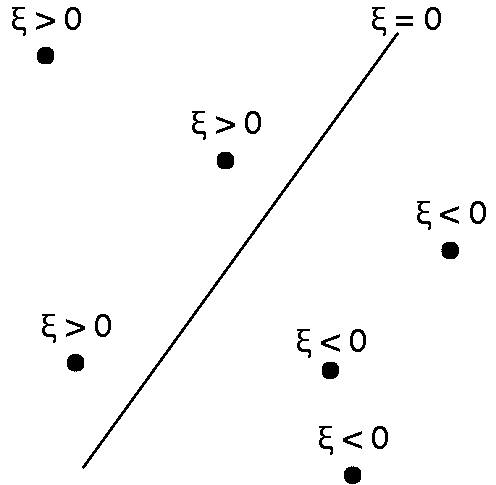
\includegraphics[width=0.45\textwidth]{tex/images/activation-vis}
\caption{Visualization of binary step activation function, which defines a separation hyperplane in n-dimensional space.}
\end{figure}

\noindent
Some desirable properties of an activation function include: \textbf{TODO}\footnote{\url{https://en.wikipedia.org/wiki/Activation_function\#Comparison_of_activation_functions}}

\begin{itemize}

\item \textit{non-linearity} - in order to map more complex functions (allows universal function approximations)
\item \textit{continuous differentiability} - necessity for gradient-based optimization methods
\item \textit{range} - for infinite range, training is generally more efficient
\item \textit{monotonicity} - the error surface associated with a single-layer models is guaranteed to be convex
\item \textit{approximates identity near the origin} - initial weights can be randomized with small differences around the origin

\end{itemize}

Here are some examples of activation functions:

\textbf{TODO activation description}
\textbf{TODO} - cite \url{https://towardsdatascience.com/activation-functions-and-its-types-which-is-better-a9a5310cc8f}

\subsection*{Identity}

\begin{figure}[H]
\raggedright
\begin{subfigure}{.25\textwidth}
  \centering
  \[ f(x) = x \]
\end{subfigure}%
\begin{subfigure}{.25\textwidth}
  \centering
  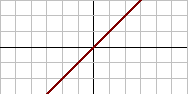
\includegraphics[width=\textwidth]{tex/images/activation/identity}
\end{subfigure}
\end{figure}

\noindent
Effectively remain the potential unchanged. 

\subsection*{Binary step}

\begin{figure}[H]
\raggedright
\begin{subfigure}{.35\textwidth}
  \centering
   \[
f(x) = \begin{cases}
       0 & x < 0 \\
       1 & x \geq 0 \\
     \end{cases} \]
\end{subfigure}%
\begin{subfigure}{.25\textwidth}
  \centering
  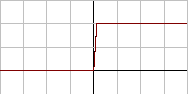
\includegraphics[width=\textwidth]{tex/images/activation/binstep}
\end{subfigure}
\end{figure}

\noindent
Basic activation function, transforms potential into a binary signal. However, this function is not differentiable.
      
\subsection*{Sigmoid}

\begin{figure}[H]
\raggedright
\begin{subfigure}{.28\textwidth}
  \centering
  \[ f(x) = \frac{1}{1 + e^{-x}} \]
\end{subfigure}%
\begin{subfigure}{.25\textwidth}
  \centering
  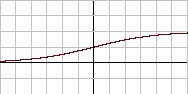
\includegraphics[width=\textwidth]{tex/images/activation/sigmoid}
\end{subfigure}
\end{figure}

\noindent
Smoothened binary step activation function, maps a real value potential into $(0,1)$ range. It introduces non-linearity. One of the most popular functions in the ANN's, mainly in the early era of machine learning. It suffers from vanishing gradient problem\footnote{describe} \textbf{TODO} and have slow convergence. Furthermore, it is not zero centered, which make optimization harder.
 
\subsection*{TanH}

\begin{figure}[H]
\raggedright
\begin{subfigure}{.5\textwidth}
  \centering
  \[ f(x) = tanh(x) = \frac{(e^x - e^{-x})}{(e^x + e^{(-x)})} \]
\end{subfigure}%
\begin{subfigure}{.25\textwidth}
  \centering
  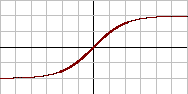
\includegraphics[width=\textwidth]{tex/images/activation/tanh}
\end{subfigure}
\end{figure}

\noindent
Unlike sigmoid, hyperbolic tangent is zero centered. It usually performs better than sigmoid. However, it stills suffers from vanishing gradient problem.

\subsection*{Rectified linear unit (ReLU)}

\begin{figure}[H]
\raggedright
\begin{subfigure}{.35\textwidth}
  \centering
   \[
f(x) = \begin{cases}
       0 & x < 0 \\
       x & x \geq 0 \\
     \end{cases} \]  
\end{subfigure}%
\begin{subfigure}{.25\textwidth}
  \centering
  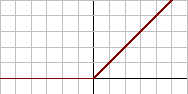
\includegraphics[width=\textwidth]{tex/images/activation/relu}
\end{subfigure}
\end{figure}

\noindent
One of the most popular function in the recent years. As opposed to previous ones, it does not have an issue with vanishing gradient. It is simple and efficient. The limitation is that it should only be used within hidden layers of a model, often combined with softmax in the output layer. It turned out to be very useful in deep learning, where traditional activation functions struggle. For example in \cite{relu_faster}, the convolutional network was able to converge six times faster with ReLU, than with tanh.

\subsection*{Leaky ReLU}

\begin{figure}[H]
\raggedright
\begin{subfigure}{.38\textwidth}
  \centering
  \[
f(x) = \begin{cases}
       0.01x & x < 0 \\
       1 & x \geq 0 \\
     \end{cases} \]  
\end{subfigure}%
\begin{subfigure}{.25\textwidth}
  \centering
  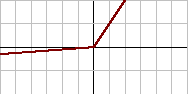
\includegraphics[width=\textwidth]{tex/images/activation/lrelu}
\end{subfigure}
\end{figure}

\noindent
One issue present in ReLU is that it allows the gradient to die off, which is not necessarily a bad thing, though it may result in dead neurons that will never activate on specific data points. To counter this, leaky ReLU's were introduced. To keep the updates alive, they add a small slope into their negative parts (usually with the factor of around 0.01).
   
\subsection*{Randomized ReLU}

\begin{figure}[H]
\raggedright
\begin{subfigure}{.35\textwidth}
  \centering
  \[
f(r, x) = \begin{cases}
       rx & x < 0 \\
       1 & x \geq 0 \\
     \end{cases} \] 
\end{subfigure}%
\begin{subfigure}{.25\textwidth}
  \centering
  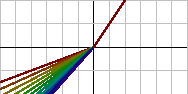
\includegraphics[width=\textwidth]{tex/images/activation/rlrelu}
\end{subfigure}
\end{figure}

\noindent
Another variant of ReLU randomizes the factor in leaky ReLU's.

\subsection*{Softmax}

\begin{figure}[H]
\raggedright
\begin{subfigure}{.25\textwidth}
  \centering
  \[ f(x_j) = \frac{e^{x_j}}{\sum_i e^{x_i}} \]
\end{subfigure}%
\begin{subfigure}{.25\textwidth}
  \centering
  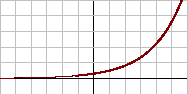
\includegraphics[width=\textwidth]{tex/images/activation/softmax}
\end{subfigure}
\end{figure}

\noindent
Softmax is usually used alongside the ReLU's in the output layer of a deep neural network. It has two nice properties:

\begin{itemize}

\item each value ranges in $[0, 1]$
\item the sum of all values is always 1

\end{itemize}

This is useful when modeling a particular probability distribution. It is used as the estimate of the class distribution for a given input.

\subsection*{Maxout}

\textbf{TODO}

\section{Artificial neural network}

Artificial neural network or feed-forward neural network is a directed acyclic graph of artificial neurons organized into several layers, where the following holds:

\begin{itemize}

\item the first layer is called the \textit{input layer}, and the output of neurons is equal to the input vector $\overrightarrow{X}$

\item the last layer is called the \textit{output layer}, and it provides the output $\overrightarrow{Y}$

\item the other layers are called the \textit{hidden layers}

\item outputs of each neuron (except for the output layer) serve as inputs of neurons in the higher layer

\item every two neighboring layers $i$ and $i+1$ make a complete bipartite graph

\item no non-neighboring layers have a connection between them

\end{itemize}

\noindent
In this section we are going to use the following terminology:

\begin{itemize}
  \item every neuron is represented as a distinct natural number (i.e neuron 1, 2, and so forth)
  \item $\xi_i$ is the inner potential of the neuron $i$
  \item $y_i$ is the output of the neuron $i$
  \item $w_{ji}$ is the weight from neuron $i$ to neuron $j$
  \item $j_{\leftarrow}$ is the set of all neurons $i$ such that there exist an edge $w_{ji}$
  \item $j_{\rightarrow}$ is the set of all neurons $i$ such that there exist an edge $w_{ij}$

\end{itemize}

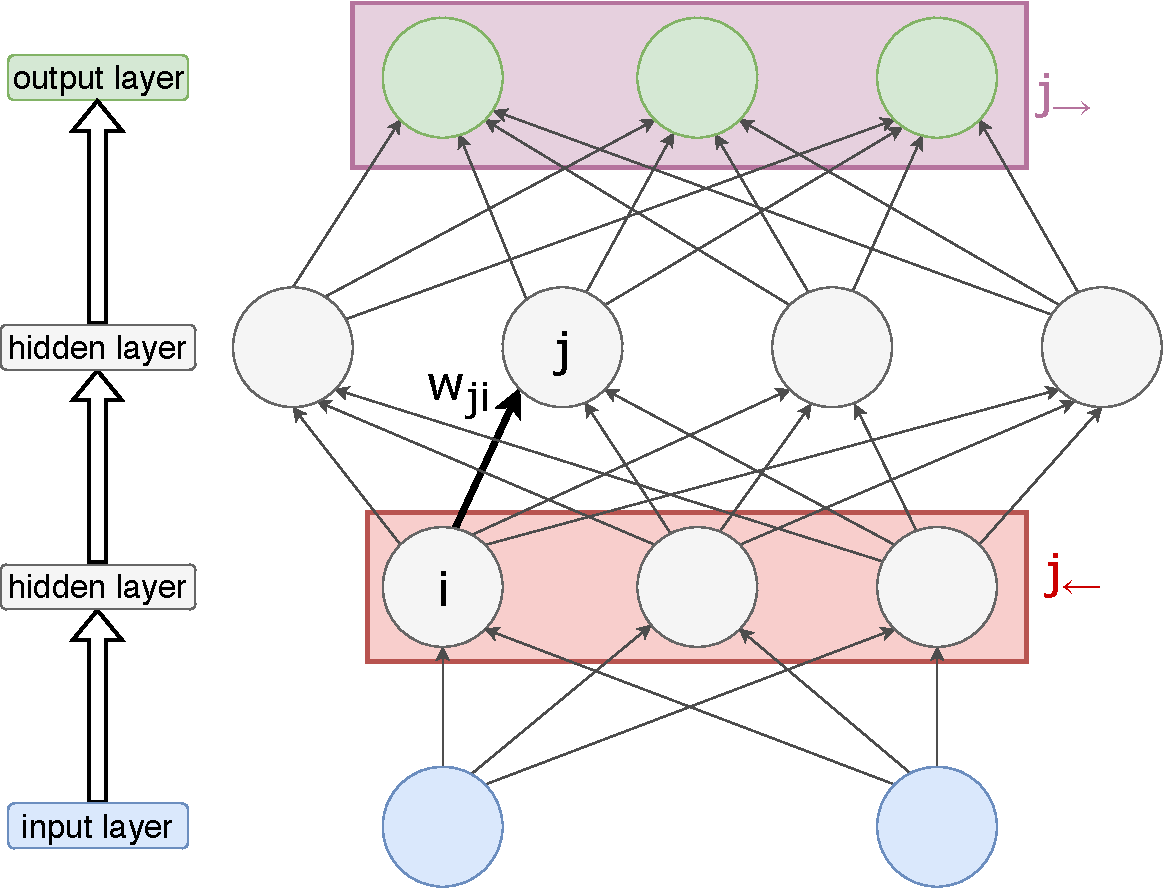
\includegraphics[width=0.8\textwidth]{tex/images/ann}

The neural network is continuously evolving, the states and connections of neurons are changing, weights are adapting. In term of these changes within a period, we can divide the network dynamics into three subcategories:

\begin{itemize}
  \item \textit{organizational} - change in topology
  \item \textit{active} - change in state
  \item \textit{adaptive} - change in configuration
\end{itemize}

\subsection*{Active dynamics}

Initially are all weights set randomly. The values in the input layer are set to the input vector $\overrightarrow{X}$. The forward propagation algorithm is then applied. Starting from the lowest layer, each layer using the output from the previous one updates its neurons. Neuron $j$ updates its inner potential:

$$ \xi_j = w_0 + \sum_{i \in j_{\leftarrow} w_{ji} y_i} $$

The output of neuron $j$ is $y_j = \sigma_j (\xi_j)$. The exception is the input layer, where $y_j = \xi_j$.

\subsection*{Adaptive dynamics}

\section{loss}
cross entropy
\section{gradient descend + backprop}
\section{DeepNN}
\section{problems}
vanishing gradient problem
dead neurons (RELU)
\section{Technizues}
dropout
\section{other ML models}

As this thesis focuses mostly on NN, we will just mention other used models.



